\section{Conclusion et perspectives}

% \begin{frame}{Conclusion}{Éditeur collaboratif Web décentralisé}
  
%   \begin{center}
%     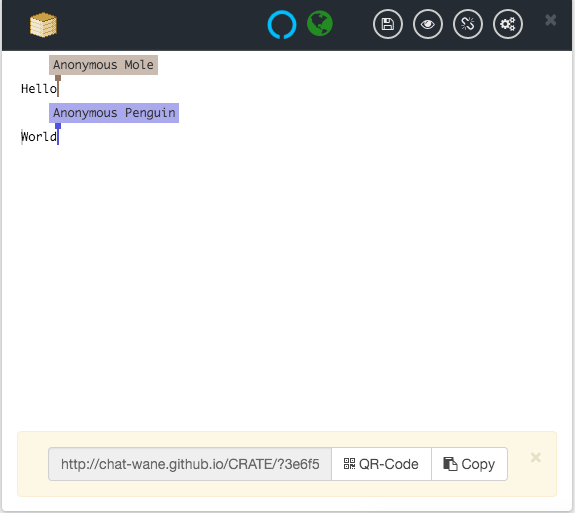
\includegraphics[width=0.85\textwidth]{img/cratescreenshot.png}
%   \end{center}

% \end{frame}


\begin{frame}{Conclusion}

  \begin{enumerate}
  \item \textbf{taille des messages :} Fonction d'allocation d'identifiants
    polylogarithmique par rapport au nombre d'insertions dans la séquence
    \vspace{0.2cm}
  \item \textbf{nombre de messages :} Protocole d'échantillonnage adaptatif
    fournissant des vues logarithmiques par rapport à la taille du réseau
  \end{enumerate}

  \vspace{1cm}
  \large
  \begin{itemize}
  \item [$\Rightarrow$] \textbf{Éditeur collaboratif Web décentralisé supportant les
    groupes d'utilisateurs de toute taille.}
  \end{itemize}

\end{frame}


% \begin{frame}{Conclusion}{Architecture}
% %  \hspace{-1cm}

% %  \begin{minipage}{0.47\textwidth}
%     \begin{center}
%       \begin{tikzpicture}[scale=0.8]

\newcommand\X{25pt}
\newcommand\Y{20pt}

\newcommand\LIGHTGRAY{gray!20}
\newcommand\MEDIUMGRAY{gray!40}

\tiny
%% communication
\draw[rounded corners=2mm, color=\MEDIUMGRAY, fill=white](0pt, 0pt)+(-4*\X,-\Y)rectangle+(4*\X,\Y);
\draw(4*\X, \Y)node[anchor=north east]{\textbf{communication}};

\draw[fill=white](-2*\X, -0.25*\Y)
node{dissémination}+(-0.85*\X,-0.5*\Y)rectangle+(0.85*\X,0.5*\Y);
\draw[fill=white, very thick, draw=darkblue]( 0*\X, 0.25*\Y)
node[align=center]{\DARKBLUE{appartenance}}+(-0.85*\X,-0.5*\Y)rectangle+(0.85*\X,0.5*\Y);
\draw[fill=white]( 2*\X, -0.25*\Y)
node{monodiffusion}+(-0.85*\X,-0.5*\Y)rectangle+(0.85*\X,0.5*\Y);

\draw[<-](-0.85*\X, 0.25*\Y)--(-1.15*\X, -0.25*\Y);
\draw[<-](0.85*\X, 0.25*\Y)--(1.15*\X, -0.25*\Y);

%% causality
\draw[rounded corners=2mm, color=\MEDIUMGRAY, fill=\LIGHTGRAY](0pt, -2*\Y)+(-4*\X,-\Y)rectangle+(4*\X,\Y);
\draw(4*\X, -\Y)node[anchor=north east]{\textbf{causalité}};

\draw[fill=\LIGHTGRAY](-2*\X, -2*\Y)
node[align=center]{détection\\[-1mm]des relations\\[-1mm]causales}
+(-1.0*\X,-0.6*\Y)rectangle+(1.0*\X,0.6*\Y);
\tiny
\draw[->, thick](-1.5*\X, -0.75*\Y) -- node[anchor=west]{reçoit}
(-1.5*\X, -1.4*\Y);
\draw[<-, thick](-2.5*\X, -0.75*\Y) -- node[anchor=east]{envoie}
(-2.5*\X, -1.4*\Y);
\tiny
\draw[<->]( 2*\X, -0.75*\Y)--( 1*\X, -2.5*\Y);

%% sequence structure
\draw[rounded corners=2mm, color=\MEDIUMGRAY, fill=white](0pt, -4*\Y)+(-4*\X,-\Y)rectangle+(4*\X,\Y);
\draw(4*\X, -3*\Y)node[anchor=north east, align=right]
{\textbf{structure}\\\textbf{pour}\\\textbf{séquences}};

\draw[fill=white, shading=axis,top color=\LIGHTGRAY, bottom color=white, shading angle=0](1*\X, -3*\Y)
node{anti-entropie}+(-0.95*\X,-0.5*\Y) rectangle +(0.95 *\X, 0.5*\Y);
\draw[fill=white, very thick, draw=darkblue](-2*\X, -4*\Y)
node{\DARKBLUE{réplique}}+(-0.75*\X,-0.5*\Y) rectangle +(0.75 *\X, 0.5*\Y);

\draw[->] (0.05*\X, -2.75*\Y)--(-1*\X,-2*\Y);
\draw[->] (0.05*\X, -3.25*\Y)--(-1.25*\X,-4*\Y);
\tiny
\draw[<-, thick] (-1.5*\X, -3.5*\Y)--node[anchor=west]{délivre}(-1.5*\X, -2.6*\Y);
\draw[->, thick] (-2.5*\X, -3.5*\Y)--node[anchor=east]{décore}(-2.5*\X, -2.6*\Y);
\tiny
%% gui
\draw[rounded corners=2mm, color=\MEDIUMGRAY, fill=\LIGHTGRAY](0pt, -6*\Y)+(-4*\X,-\Y)rectangle+(4*\X,\Y);
\draw(4*\X, -5*\Y)node[anchor=north east, align=right]
{\textbf{interface}\\\textbf{utilisateur}};
\draw[fill=\LIGHTGRAY](0pt,-6*\Y)
node{éditeur web}+(-0.85*\X,-0.5*\Y) rectangle +(0.85 *\X, 0.5*\Y);

%%\draw[<->] (-2*\X, -4.5*\Y) -- (0*\X, -5.5*\Y);
\tiny
\draw[->, thick] (-1.80*\X, -4.5*\Y)--node[anchor=west]{notifie}(-0.85*\X, -5.75*\Y);
\draw[<-, thick] (-2.20*\X, -4.5*\Y)--node[anchor=east]{met à jour}(-0.85*\X, -6.25*\Y);
\tiny
\end{tikzpicture}
%     \end{center}
% %  \end{minipage}
    
%     Le trafic croît 
%     \begin{itemize}
%     \item logarithmiquement par rapport au nombre de collaborateurs grâce à \SPRAY;
%     \item polylogarithmiquement par rapport au nombre d'insertions dans le
%       document grâce à \LSEQ.
%     \end{itemize}

%  \hfill
  % \hspace{0.5cm}
  % \begin{minipage}{0.47\textwidth}
  %   \begin{center}
  %     
\begin{tikzpicture}[scale=1.3]

  \newcommand\X{35pt}
  \newcommand\Y{-35pt}
  
%  \small

%  \draw (-35-2*\X, 30pt);

  
%  \draw[fill=white] (-2*\X, 1.5*\Y) 
%  node{
\includegraphics[width=12pt]{img/crateicon.png}};
  % node{$e_9$}; % +(-5pt,-5pt) rectangle +(5pt,5pt);
  % \only<3>{
  %   \draw[<->, densely dashed, color=darkblue, very thick]
  %   (-2*\X, 5+1.5*\Y) -- node[anchor=east]{\DARKBLUE{rejoint}} (-2*\X, -5pt);
  % }
  % \only<4-5>{
  %   \draw[<->, densely dashed, color=darkblue, very thick]
  %   (-2*\X, 5+1.5*\Y) -- (-2*\X, -5pt);
  % }
  % \only<4>{
  %   \draw[->, very thick] (5-2*\X, 10+1.5*\Y) -- (5-2*\X, -10pt);
  %   \draw[->, very thick] (20-2*\X, -10pt) -- (-12pt, \Y);
  % }
  % \only<5>{
  %   \draw[<-, very thick] (5-2*\X, 10+1.5*\Y) -- (5-2*\X, -10pt);
  %   \draw[<-, very thick] (20-2*\X, -10pt) -- (-12pt, \Y);
  % }

  % \only<6->{
  %   \draw[<->, very thick](5-2*\X,1.5*\Y) -- (-5pt, -3+ \Y);
  % }


  % \only<8->{
  %   \draw[<->, very thick](5-2*\X, -3+1.5*\Y ) -- (-5+3*\X ,1*\Y);
  % }

  %   \draw[fill=white] (-2*\X, 0) node{$mediateur_1$} +(-20pt,
  %   -5pt)rectangle+(18pt, 5pt);
  %   \only<2->{
  %   \draw[<->, densely dashed, color=darkblue, very thick]
  %   (20-2*\X, 0) -- node[anchor=south]{\DARKBLUE{partage}} (-5+\X, 0);
  %   \draw[<->, densely dashed, color=darkblue, very thick]
  %   (20-2*\X, -5pt) -- (-5pt, \Y);
  % }
  
  %   \draw[fill=white] (-2*\X, 3*\Y) node{$mediateur_2$} +(-18pt, -5pt)rectangle+(18pt, 5pt);
  % \only<2->{
  %   \draw[<->, densely dashed, color=darkblue] (20-2*\X, 3*\Y) -- (-5+\X, 3*\Y);
  %   \draw[<->, densely dashed, color=darkblue] (20-2*\X, 5+3*\Y) -- (-5pt, 2*\Y);
  % }

  \draw[fill=white] (\X, 0)node{
\includegraphics[width=18pt]{img/firefox.png}};
  % node{$e_1$}+(-5pt, -5pt)rectangle+(5pt, 5pt);
  \draw[fill=white] (2*\X, 0)node{
\includegraphics[width=18pt]{img/chrome.png}};
  % {$e_2$}+(-5pt, -5pt)rectangle+(5pt, 5pt);
  \draw[fill=white] (3*\X, \Y)node{
\includegraphics[width=18pt]{img/chrome.png}};
  % ;{$e_3$}+(-5pt, -5pt)rectangle+(5pt, 5pt);
  \draw[fill=white] (3*\X, 2*\Y)node{
\includegraphics[width=18pt]{img/firefox.png}};
  % {$e_4$}+(-5pt, -5pt)rectangle+(5pt, 5pt);
  \draw[fill=white] (2*\X, 3*\Y)node{
\includegraphics[width=18pt]{img/chrome.png}};
  % {$e_5$}+(-5pt, -5pt)rectangle+(5pt, 5pt);
  \draw[fill=white] (1*\X, 3*\Y)node{
\includegraphics[width=18pt]{img/firefox.png}};
  % {$e_6$}+(-5pt, -5pt)rectangle+(5pt, 5pt);
  \draw[fill=white] (0 , 2*\Y)node{
\includegraphics[width=18pt]{img/firefox.png}};
  % {$e_7$}+(-5pt, -5pt)rectangle+(5pt, 5pt);
  % \draw[fill=white] (0 , \Y)+(-55pt, -10pt)rectangle+(5pt, 10pt);
  \draw[fill=white](0,\Y)node{
\includegraphics[width=18pt]{img/chrome.png}};
  % {$e_8$}+(-5pt, -5pt)rectangle+(5pt, 5pt);


  \draw[->] (\X, 0)--(\X, 5+3*\Y); %% p1 p6
  \draw[->] (-5+2*\X, 0)--(5+\X, 0); %% p2 p1
  \draw[->] (2*\X, 0) -- (-5+3*\X, \Y); %% p2 p3
  \draw[->] (2*\X, 0) -- (-5+3*\X, 2*\Y); %% p2 p4
  \draw[->] (3*\X, 5+\Y) -- ( 5+2*\X, 0); %% p3 p2
  \draw[->] (3*\X, \Y) -- (5pt, 2*\Y); %% p3 p7
  \draw[->] (3*\X, \Y) -- (2*\X, 5+3*\Y); %% p3 p5
  \draw[->] (3*\X, 2*\Y) -- (5pt, 2*\Y); %% p4 p7
  \draw[->] (3*\X, 2*\Y) -- (5pt, \Y); %% p4 p8
  \draw[->] (2*\X, 3*\Y) -- (\X, -5pt); %% p5 p1
  \draw[->] (5+2*\X, 3*\Y) -- (3*\X, -5+ 2*\Y); %% p5 p4
  \draw[->] (-5+\X, 3*\Y) -- (0pt, -5+2*\Y); %% p6 p7
  \draw[->] (0pt, 2*\Y) -- (-5+3*\X, \Y); %% p7 p3
  \draw[->] (0pt, 2*\Y) -- (\X, -5pt); %% p7 p1
  \draw[->] (0pt, \Y) -- (2*\X, -5pt); %% p8 p2
  \draw[->] (0pt, \Y) -- (\X, 5+3*\Y); %% p8 p6
  \draw[->] (0pt, \Y) -- (-5+3*\X, \Y); %% p8 p3

  \draw[fill=white] (\X, 0)node{
\includegraphics[width=12pt]{img/crateicon.png}};
  \draw[fill=white] (2*\X, 0)node{
\includegraphics[width=12pt]{img/crateicon.png}};
  \draw[fill=white] (3*\X, \Y)node{
\includegraphics[width=12pt]{img/crateicon.png}};
  \draw[fill=white] (3*\X, 2*\Y)node{
\includegraphics[width=12pt]{img/crateicon.png}};
  \draw[fill=white] (2*\X, 3*\Y)node{
\includegraphics[width=12pt]{img/crateicon.png}};
  \draw[fill=white] (1*\X, 3*\Y)node{
\includegraphics[width=12pt]{img/crateicon.png}};
  \draw[fill=white] (0, 2*\Y)node{
\includegraphics[width=12pt]{img/crateicon.png}};
  \draw[fill=white] (0, \Y)node{
\includegraphics[width=12pt]{img/crateicon.png}};


  \only<2->{
    \draw (0pt, \Y) node{\textbf{A}};
  }

  \only<3>{
    \draw[->, very thick] (0pt, \Y) -- (2*\X, -5pt); %% p8 p2
    \draw[->, very thick] (0pt, \Y) -- (\X, 5+3*\Y); %% p8 p6
    \draw[->, very thick] (0pt, \Y) -- (-5+3*\X, \Y); %% p8 p3

    \draw[fill=white] (0*\X, \Y)node{
\includegraphics[width=12pt]{img/crateicon.png}};
    \draw (0pt, \Y) node{\textbf{A}};
  }
  
  \only<3->{
    \draw (2*\X, 0pt) node{\textbf{A}};
    \draw (\X, 3*\Y) node{\textbf{A}};
    \draw (3*\X, \Y) node{\textbf{A}};
  }
  
  \only<4>{
    \draw[->, very thick] (-5+2*\X, 0)--(5+\X, 0); %% p2 p1
    \draw[->, very thick] (2*\X, 0) -- (-5+3*\X, \Y); %% p2 p3
    \draw[->, very thick] (2*\X, 0) -- (-5+3*\X, 2*\Y); %% p2 p4
    \draw (2*\X, 0)node{
\includegraphics[width=12pt]{img/crateicon.png}}node{\textbf{A}};
    
    \draw[->, very thick] (-5+\X, 3*\Y) -- (0pt, -5+2*\Y); %% p6 p7
    \draw (\X, 3*\Y)node{
\includegraphics[width=12pt]{img/crateicon.png}}node{\textbf{A}};

    \draw[->, very thick] (3*\X, 5+\Y) -- ( 5+2*\X, 0); %% p3 p2
    \draw[->, very thick] (3*\X, \Y) -- (5pt, 2*\Y); %% p3 p7
    \draw[->, very thick] (3*\X, \Y) -- (2*\X, 5+3*\Y); %% p3 p5
    \draw (3*\X, \Y)node{
\includegraphics[width=12pt]{img/crateicon.png}}node{\textbf{A}};
  }

  \only<4->{
    \draw (\X, 0) node{\textbf{A}};
    \draw (3*\X, \Y) node{\textbf{A}};
    \draw (3*\X, 2*\Y) node{\textbf{A}};

    \draw (2*\X, 0pt) node{\textbf{A}};
    \draw (0pt, 2*\Y) node{\textbf{A}};
    \draw (2*\X, 3*\Y) node{\textbf{A}};
  }

  \only<5>{
    \draw[->, very thick] (\X, 0)--(\X, 5+3*\Y); %% p1 p6
    \draw (\X, 0)node{
\includegraphics[width=12pt]{img/crateicon.png}}node{\textbf{A}};

    \draw[->, very thick] (3*\X, 2*\Y) -- (5pt, 2*\Y); %% p4 p7
    \draw[->, very thick] (3*\X, 2*\Y) -- (5pt, \Y); %% p4 p8
     \draw (3*\X, 2*\Y)node{
\includegraphics[width=12pt]{img/crateicon.png}}node{\textbf{A}}; 
    \draw[->, very thick] (2*\X, 3*\Y) -- (\X, -5pt); %% p5 p1
    \draw[->, very thick] (5+2*\X, 3*\Y) -- (3*\X, -5+ 2*\Y); %% p5 p4
    \draw (2*\X, 3*\Y)node{
\includegraphics[width=12pt]{img/crateicon.png}}node{\textbf{A}};
    \draw[->, very thick] (0pt, 2*\Y) -- (-5+3*\X, \Y); %% p7 p3
    \draw[->, very thick] (0pt, 2*\Y) -- (\X, -5pt); %% p7 p1
    \draw (0, 2*\Y)node{
\includegraphics[width=12pt]{img/crateicon.png}}node{\textbf{A}};
  };


\end{tikzpicture}
  %   \end{center}
  % \end{minipage}
%\end{frame}


% \begin{frame}{Conclusion}{Évaluation du passage à l'échelle sur Grid'5k}

%   \begin{center}
%     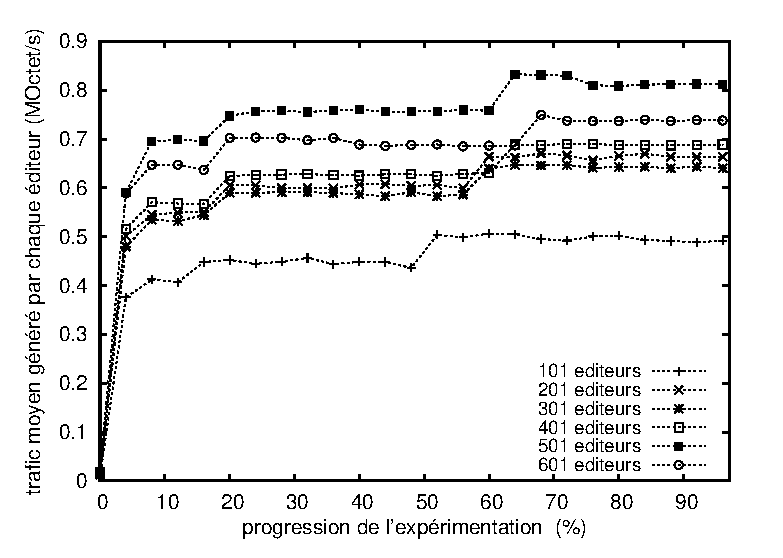
\includegraphics[width=1\textwidth]{img/editor/communication.eps}
%   \end{center}

% \end{frame}


\begin{frame}{Conclusion}{Perspectives : la fusion de réseaux}

  \begin{block}{Les réseaux fusionnant préservent leurs propriétés}
    Soit $\mathcal{N}_1,\, \mathcal{N}_2,\, \ldots ,\, \mathcal{N}_k$ des réseaux
    de taille arbitraire. On a : \vspace{-5pt}
    \begin{equation}
      \sum\limits_{i = 1}^k |\mathcal{N}_i|\ln (|\mathcal{N}_i|) < (\sum\limits_{i = 1}^k |\mathcal{N}_i|)\ln{(\sum\limits_{i=1}^k |\mathcal{N}_i|)}
    \end{equation}
    Comment adapter les nombres d'arcs effectif (à gauche) pour qu'il atteigne le
    nombre d'arcs requis (à droite)?
  \end{block}

  \begin{minipage}{0.325\textwidth}
    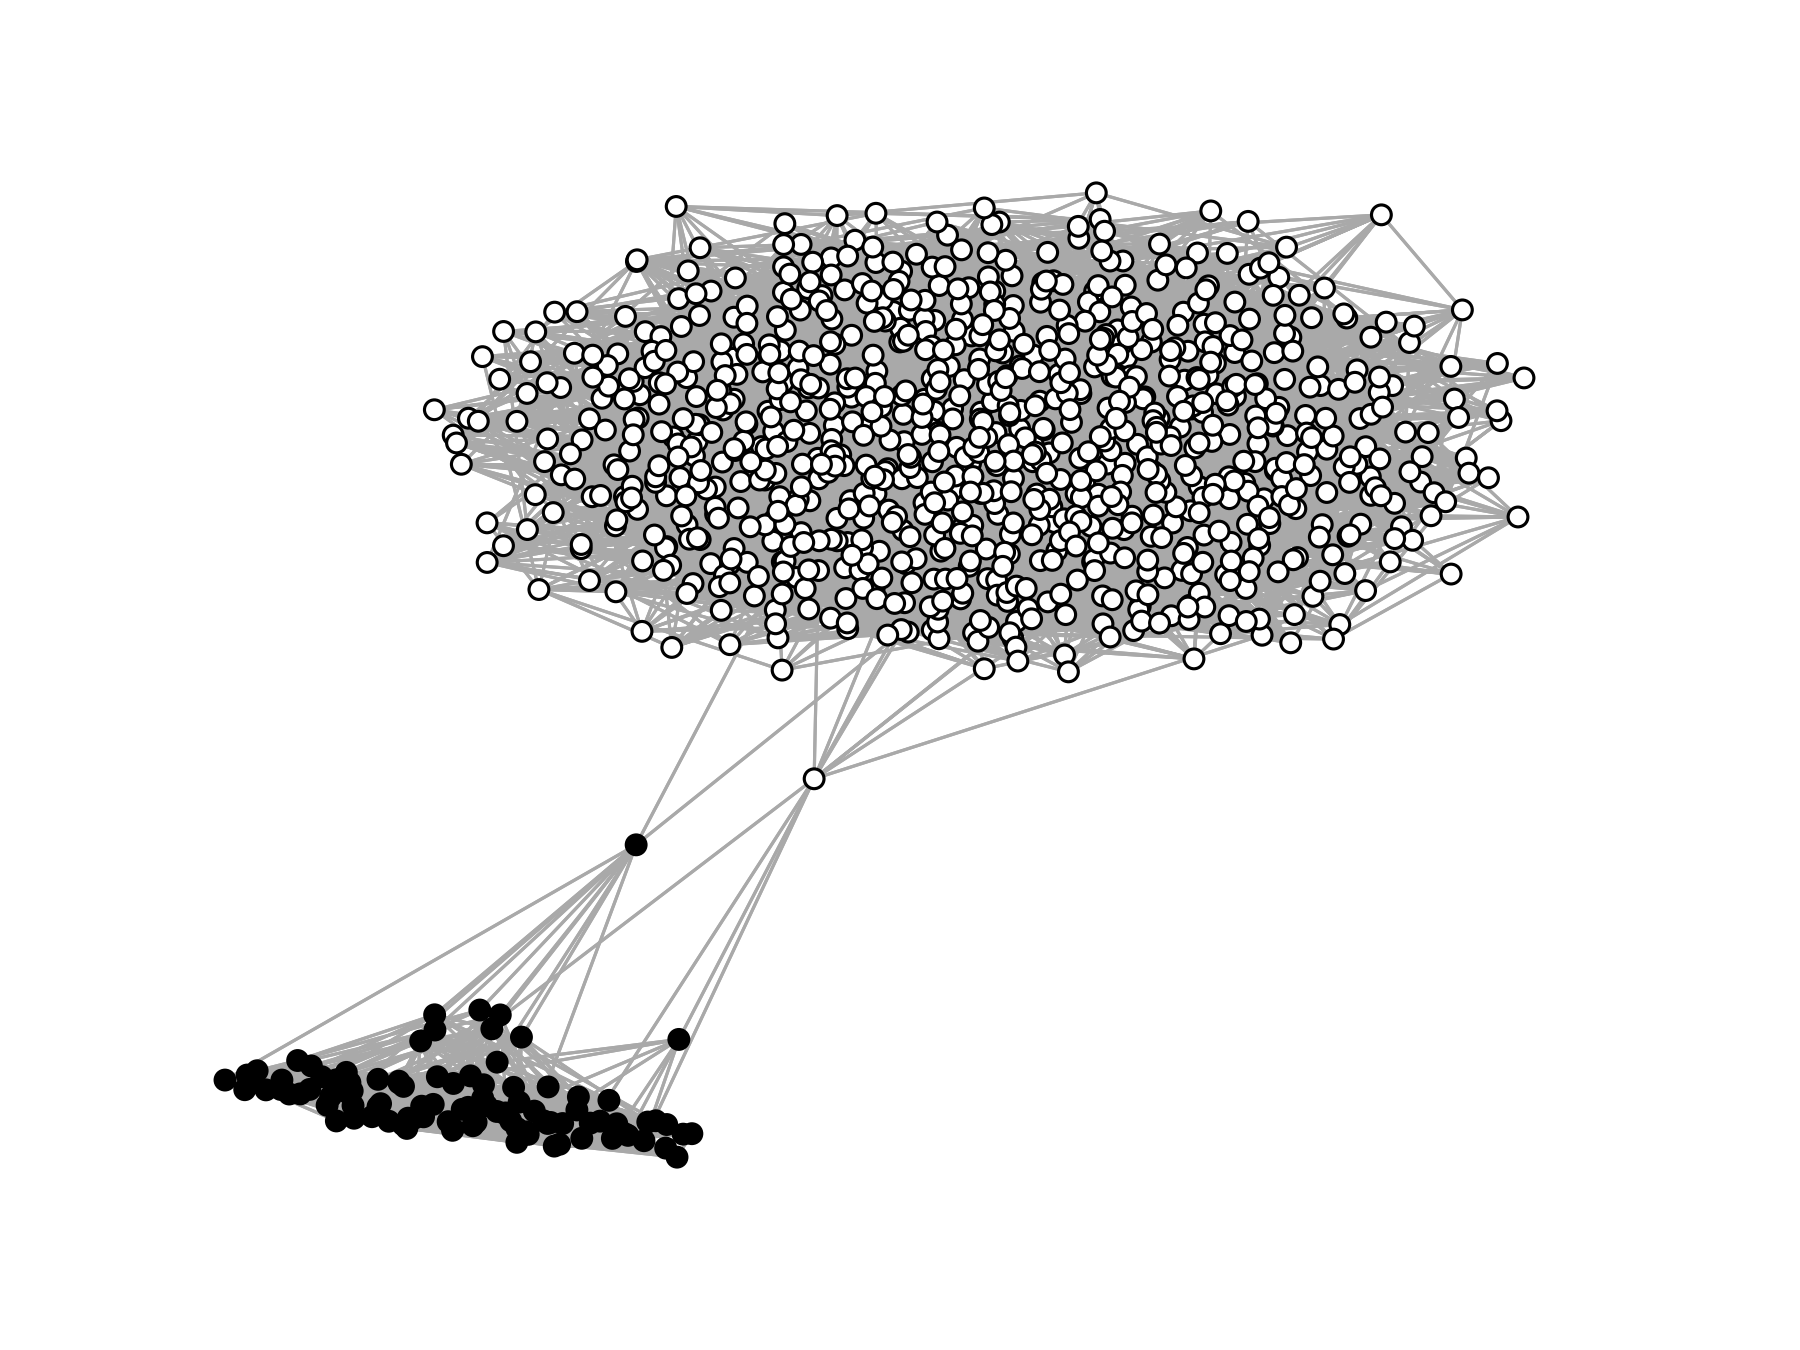
\includegraphics[width=1.2\textwidth]{img/graphA.png}
  \end{minipage}
  \begin{minipage}{0.325\textwidth}
    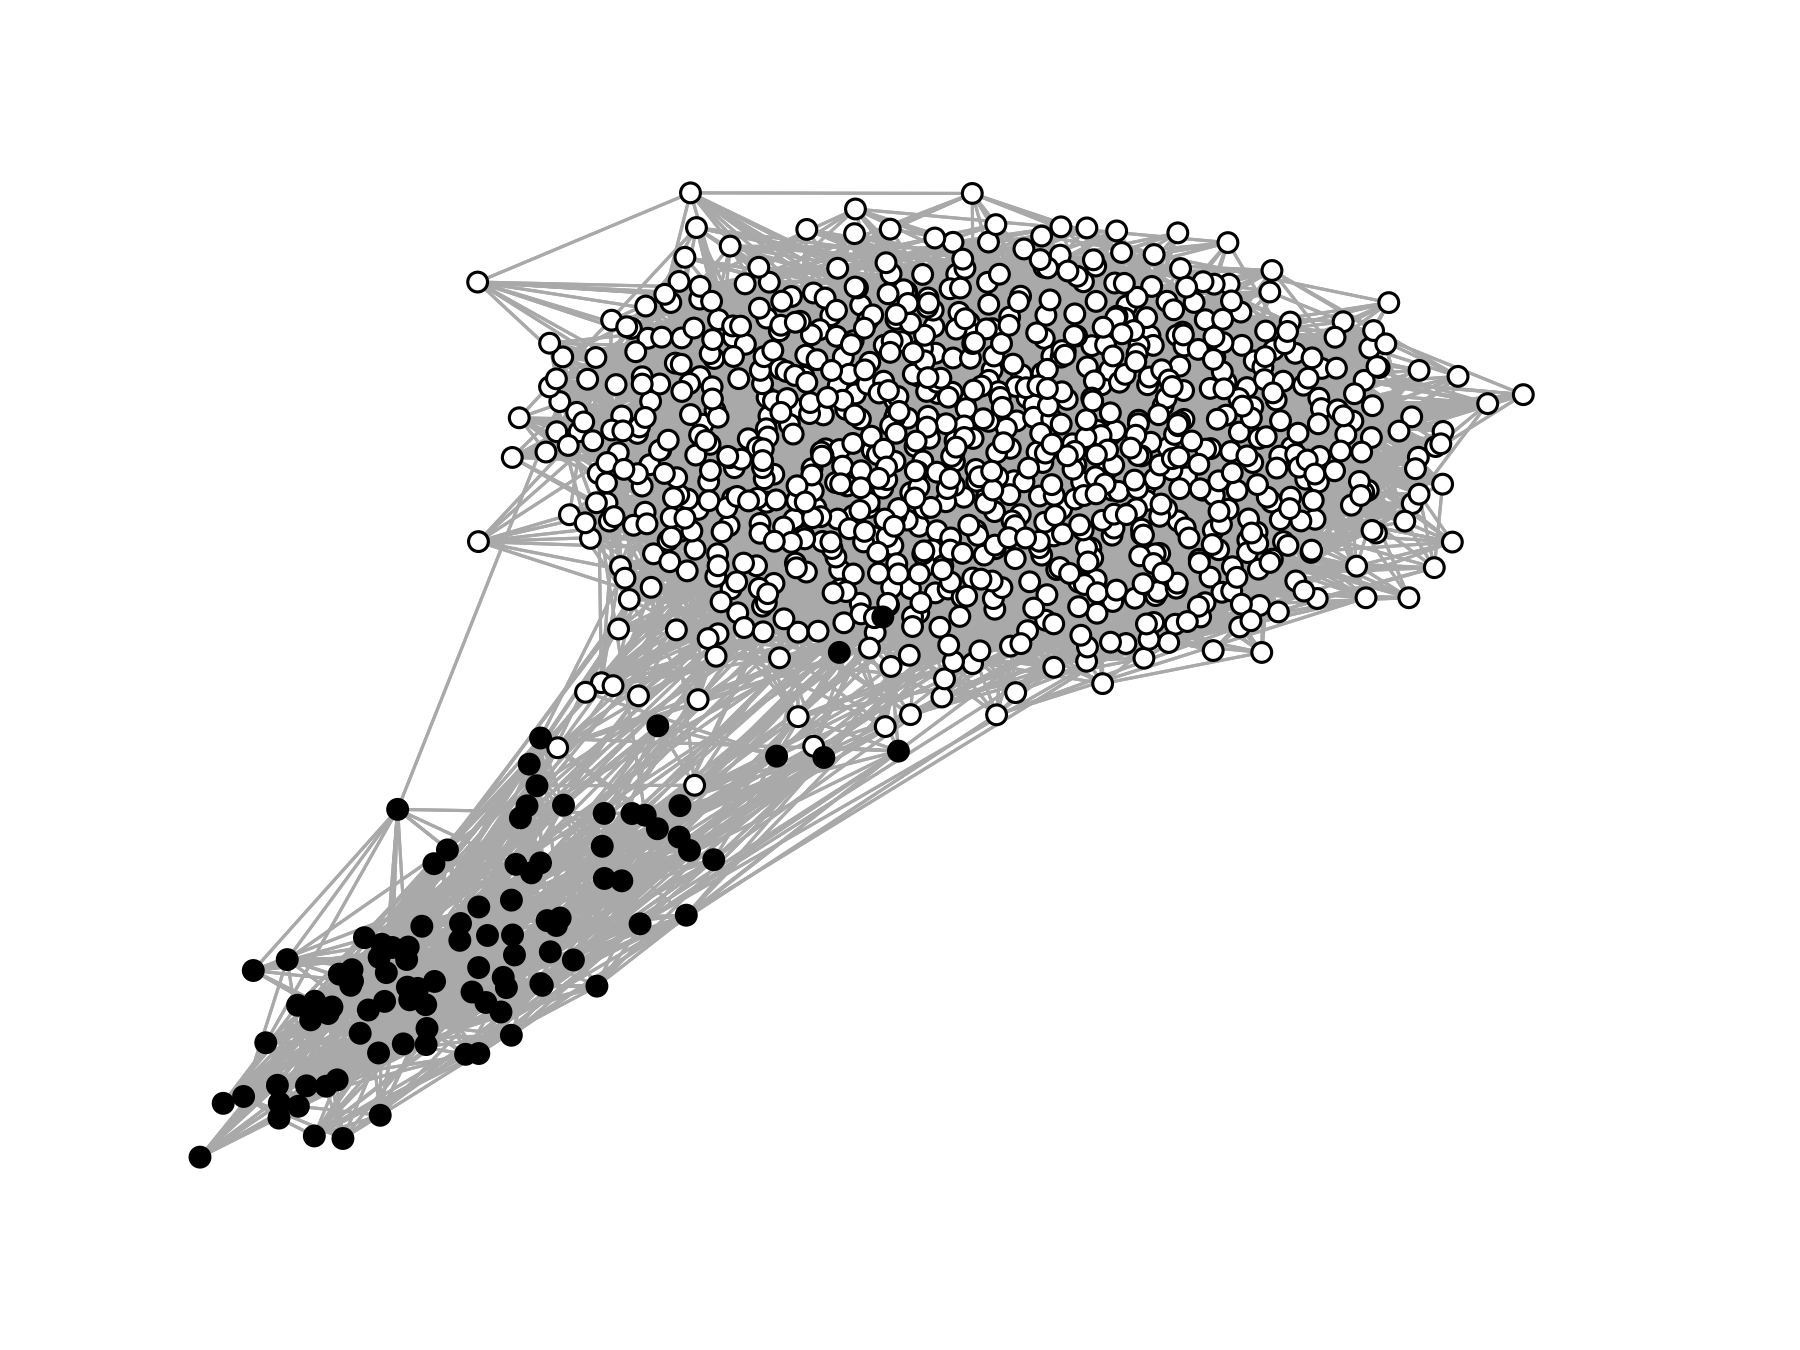
\includegraphics[width=1.2\textwidth]{img/graphB.png}
  \end{minipage}
  \begin{minipage}{0.325\textwidth}
    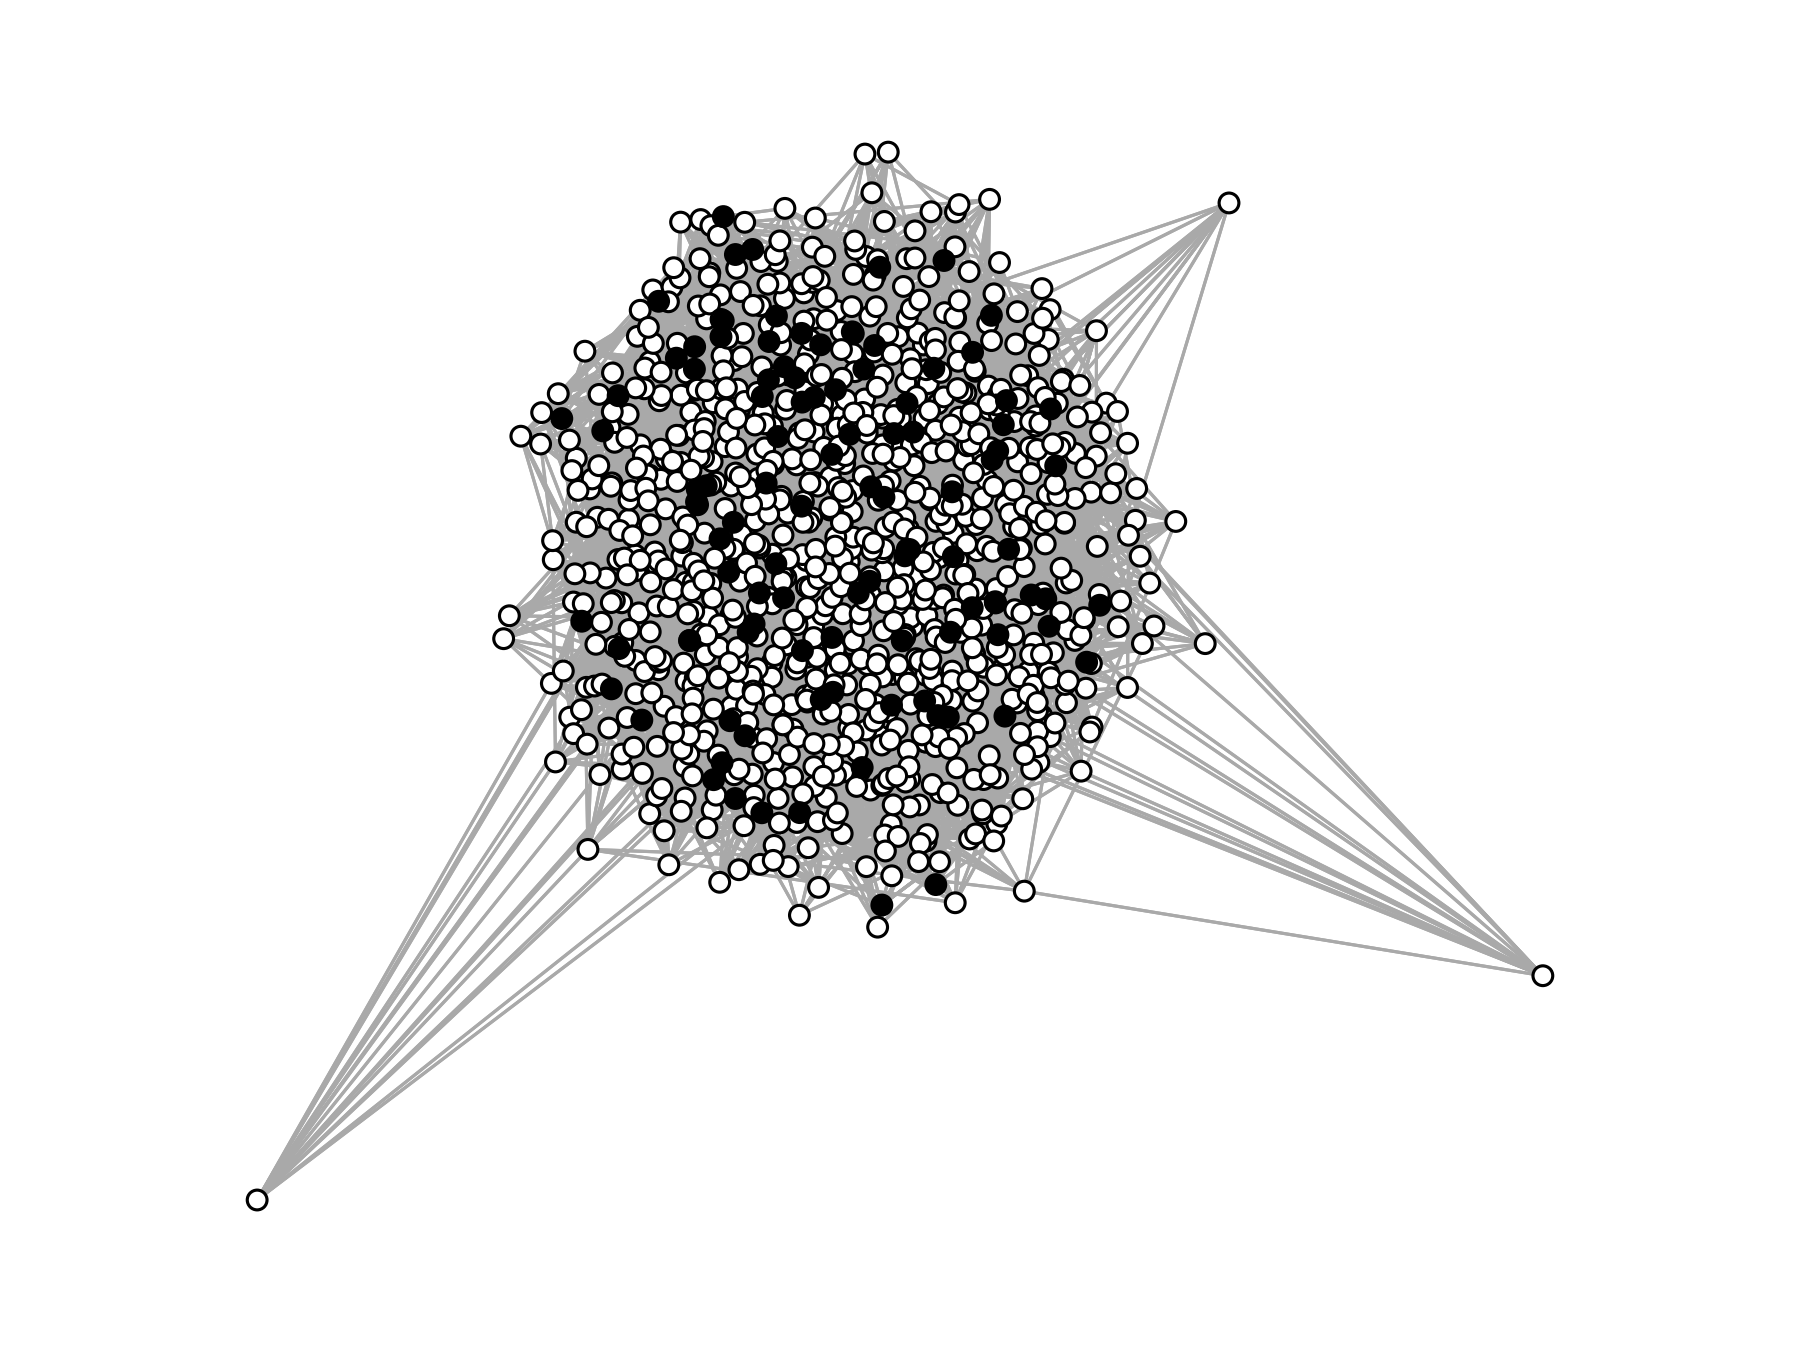
\includegraphics[width=1.2\textwidth]{img/graphC.png}
  \end{minipage}

\end{frame}

\begin{frame}{Conclusion}{Perspectives : les tables de hachage réparties}

%  \begin{minipage}{0.45\textwidth}
%  \begin{itemize}
%  \item Table de hachage répartie
%  \end{itemize}
%  \end{minipage}
%  \hfill
%  \begin{minipage}{0.45\textwidth}

  


  \begin{center}
    
\begin{tikzpicture}[scale=0.7]

  \newcommand\X{75pt};
  \newcommand\Y{75pt};

  \newcommand\1{0.865};
  \newcommand\2{0.705};
  \newcommand\3{0.5};

  \scriptsize
  \draw[fill=white, very thick, draw=darkblue]
  (1*\X, 0*\Y) node{\DARKBLUE{$n_1$}} +(-5pt,-5pt) rectangle +(5pt,5pt);
  \draw[fill=white]
  (\1*\X, \3*\Y) node{$n_2$} +(-5pt,-5pt) rectangle +(5pt,5pt);
  \draw[fill=white]
  (\2*\X, \2*\Y) node{$n_3$} +(-5pt,-5pt) rectangle +(5pt,5pt);
  \draw[fill=white]
  (\3*\X, \1*\Y) node{$n_4$} +(-5pt,-5pt) rectangle +(5pt,5pt);
  \draw[fill=white]
  (0*\X, 1*\Y) node{$n_5$} +(-5pt,-5pt) rectangle +(5pt,5pt);
  
  \draw[->, very thick, color = darkblue](1*\X, 5+0*\Y) --
  node[anchor=west]{\DARKBLUE{\textbf{plus proche}}} (\1*\X, -5+\3*\Y);
  \draw[->](-5+\1*\X, 5+\3*\Y) -- (5+\2*\X, -5+\2*\Y);
  \draw[->](-5+\2*\X, 5+\2*\Y) -- (5+\3*\X, -5+\1*\Y);
  \draw[->](-5+\3*\X, \1*\Y) -- (5+0*\X, 1*\Y);


  \draw[fill=white]
  (-\3*\X, \1*\Y) node{$n_6$} +(-5pt,-5pt) rectangle +(5pt,5pt);
  \draw[fill=white]
  (-\2*\X, \2*\Y) node{$n_7$} +(-5pt,-5pt) rectangle +(5pt,5pt);
  \draw[fill=white]
  (-\1*\X, \3*\Y) node{$n_8$} +(-5pt,-5pt) rectangle +(5pt,5pt);
  \draw[fill=white]
  (-1*\X, 0*\Y) node{$n_9$} +(-5pt,-5pt) rectangle +(5pt,5pt);

  \draw[->](-5+0*\X, 1*\Y) -- (5+-\3*\X, \1*\Y);
  \draw[->](-5-\3*\X, -5+\1*\Y) -- (5-\2*\X, 5+\2*\Y);
  \draw[->](-5-\2*\X, -5+\2*\Y) -- (5-\1*\X, 5+\3*\Y);
  \draw[->](-\1*\X, -5+\3*\Y) -- (-1*\X, 5+0*\Y);

  \draw[fill=white]
  (-\1*\X, -\3*\Y) node{$n_{10}$} +(-5pt,-5pt) rectangle +(5pt,5pt);
  \draw[fill=white]
  (-\2*\X, -\2*\Y) node{$n_{11}$} +(-5pt,-5pt) rectangle +(5pt,5pt);
  \draw[fill=white]
  (-\3*\X, -\1*\Y) node{$n_{12}$} +(-5pt,-5pt) rectangle +(5pt,5pt);
  \draw[fill=white]
  (0*\X, -1*\Y) node{$n_{13}$} +(-5pt,-5pt) rectangle +(5pt,5pt);

  \draw[->](-1*\X, -5+0*\Y) -- (-\1*\X, 5-\3*\Y);
  \draw[->](5-\1*\X, -5-\3*\Y) -- (-5-\2*\X, 5-\2*\Y);
  \draw[->](5-\2*\X, -5-\2*\Y) -- (-5-\3*\X, 5-\1*\Y);
  \draw[->](5-\3*\X, -\1*\Y) -- (-5+0*\X, -1*\Y);

  \draw[fill=white]
  (\3*\X, -\1*\Y) node{$n_{14}$} +(-5pt,-5pt) rectangle +(5pt,5pt);
  \draw[fill=white]
  (\2*\X, -\2*\Y) node{$n_{15}$} +(-5pt,-5pt) rectangle +(5pt,5pt);
  \draw[fill=white]
  (\1*\X, -\3*\Y) node{$n_{16}$} +(-5pt,-5pt) rectangle +(5pt,5pt);

  \draw[->](5+0*\X, -1*\Y) -- (-5+\3*\X, -5-\1*\Y);
  \draw[->](5+\3*\X, -\1*\Y) -- (-5+\2*\X, -5-\2*\Y);
  \draw[->](5+\2*\X, 5-\2*\Y) -- (-5+\1*\X, -5-\3*\Y);
  \draw[->](\1*\X, 5-\3*\Y) -- (1*\X, -5+0*\Y);


  \draw[<->](0*\X, -5+1*\Y) -- (0*\X, 5+-1*\Y);
  \draw[<->](-5+\1*\X, -5+\3*\Y) -- (5-\1*\X, 5-\3*\Y);
  \draw[<->](-5+\2*\X, -5+\2*\Y) -- (5-\2*\X, 5-\2*\Y);
  \draw[<->](-5+\3*\X, -5+\1*\Y) -- (5-\3*\X, 5-\1*\Y);
  \draw[<->](-5+\1*\X, 5-\3*\Y) -- (5-\1*\X, -5+\3*\Y);
  \draw[<->](-5+\2*\X, 5-\2*\Y) -- (5-\2*\X, -5+\2*\Y);
  \draw[<->](-5+\3*\X, 5-\1*\Y) -- (5-\3*\X, -5+\1*\Y);


  \draw[->] (-5+\1*\X, \3*\Y) -- (5-\2*\X , \2*\Y); %% 2-> 7
  \draw[->] (-5+\2*\X, \2*\Y) -- (5-\1*\X, \3*\Y); %% 3 -> 8
%  \draw[->] (-5+\3*\X, -5+\1*\Y) -- (5-1*\X, 5+0*\Y); %% 4 -> 9
%  \draw[->] (-5+0*\X, -5+1*\Y) -- (5-\1*\X, 5-\3*\Y); %% 5 -> 10
  \draw[->] (-\3*\X, -5+\1*\Y) -- (-\2*\X, 5-\2*\Y); %% 6 -> 11
  \draw[->] (-\2*\X, -5+\2*\Y) -- (-\3*\X, 5-\1*\Y); %% 7 -> 12
  \draw[->] (5+-\1*\X, -5+\3*\Y) -- (-5+0*\X, 5-1*\Y); %% 8 -> 13
  \draw[->] (5+-1*\X, -5+0*\Y) -- (-5+\3*\X, 5-\1*\Y); %% 9 -> 14
  \draw[->] (5-\1*\X, -\3*\Y) -- (-5+\2*\X, -\2*\Y); %% 10 -> 15
%  \draw[->] (5-\2*\X, -\2*\Y) -- (-5+\1*\X, -\3*\Y); %% 11 -> 16
  \draw[->] (5-\3*\X, 5-\1*\Y) -- (-5+1*\X, -5+0*\Y); %% 12 -> 1
%  \draw[->] (5-0*\X, 5-1*\Y) -- (-5+\1*\X, -5+\3*\Y); %% 13 -> 2
  \draw[->] (\3*\X, 5-\1*\Y) -- (\2*\X, -5+\2*\Y); %% 14 -> 3
  \draw[->] (\2*\X, 5-\2*\Y) -- (\3*\X, -5+\1*\Y); %% 15 -> 4
  \draw[->] (-5+\1*\X, 5-\3*\Y) -- (5+0*\X, -5+1*\Y); %% 16 -> 5


  \draw[<->, very thick, color = darkblue](5-\X, 0*\Y) --
  node[anchor=south west]{\DARKBLUE{\textbf{plus lointain}}}(-5+\X, 0*\Y);
  \draw[->, very thick, color = darkblue] (-5+\X, 5+0*\Y) --
  node[anchor=south]{\DARKBLUE{$\mathbf{1\over{3}}$}}(5-\3*\X, -5+\1*\Y); %% 1 -> 6
\end{tikzpicture}


%%% Local Variables:
%%% mode: latex
%%% TeX-master: "../../paper"
%%% End:

  \end{center}
%  \end{minipage}

\end{frame}

\begin{frame}{Conclusion}{Perspectives}
  \begin{itemize}
  \item Compromis entre causalité et concurrence
  \end{itemize}
\end{frame}


\begin{frame}{Conclusion}{Perspectives : O'Browser, Where Art Thou ?}

  \begin{center}
    \begin{tikzpicture}[scale=0.8]

\newcommand\X{25pt}
\newcommand\Y{20pt}

\newcommand\LIGHTGRAY{gray!20}
\newcommand\MEDIUMGRAY{gray!40}

\tiny
%% communication
\draw[rounded corners=2mm, color=\MEDIUMGRAY, fill=white](0pt, 0pt)+(-4*\X,-\Y)rectangle+(4*\X,\Y);
\draw(4*\X, \Y)node[anchor=north east]{\textbf{communication}};

\draw[fill=white](-2*\X, -0.25*\Y)
node{dissémination}+(-0.85*\X,-0.5*\Y)rectangle+(0.85*\X,0.5*\Y);
\draw[fill=white, very thick, draw=darkblue]( 0*\X, 0.25*\Y)
node[align=center]{\DARKBLUE{appartenance}}+(-0.85*\X,-0.5*\Y)rectangle+(0.85*\X,0.5*\Y);
\draw[fill=white]( 2*\X, -0.25*\Y)
node{monodiffusion}+(-0.85*\X,-0.5*\Y)rectangle+(0.85*\X,0.5*\Y);

\draw[<-](-0.85*\X, 0.25*\Y)--(-1.15*\X, -0.25*\Y);
\draw[<-](0.85*\X, 0.25*\Y)--(1.15*\X, -0.25*\Y);

%% causality
\draw[rounded corners=2mm, color=\MEDIUMGRAY, fill=\LIGHTGRAY](0pt, -2*\Y)+(-4*\X,-\Y)rectangle+(4*\X,\Y);
\draw(4*\X, -\Y)node[anchor=north east]{\textbf{causalité}};

\draw[fill=\LIGHTGRAY](-2*\X, -2*\Y)
node[align=center]{détection\\[-1mm]des relations\\[-1mm]causales}
+(-1.0*\X,-0.6*\Y)rectangle+(1.0*\X,0.6*\Y);
\tiny
\draw[->, thick](-1.5*\X, -0.75*\Y) -- node[anchor=west]{reçoit}
(-1.5*\X, -1.4*\Y);
\draw[<-, thick](-2.5*\X, -0.75*\Y) -- node[anchor=east]{envoie}
(-2.5*\X, -1.4*\Y);
\tiny
\draw[<->]( 2*\X, -0.75*\Y)--( 1*\X, -2.5*\Y);

%% sequence structure
\draw[rounded corners=2mm, color=\MEDIUMGRAY, fill=white](0pt, -4*\Y)+(-4*\X,-\Y)rectangle+(4*\X,\Y);
\draw(4*\X, -3*\Y)node[anchor=north east, align=right]
{\textbf{structure}\\\textbf{pour}\\\textbf{séquences}};

\draw[fill=white, shading=axis,top color=\LIGHTGRAY, bottom color=white, shading angle=0](1*\X, -3*\Y)
node{anti-entropie}+(-0.95*\X,-0.5*\Y) rectangle +(0.95 *\X, 0.5*\Y);
\draw[fill=white, very thick, draw=darkblue](-2*\X, -4*\Y)
node{\DARKBLUE{réplique}}+(-0.75*\X,-0.5*\Y) rectangle +(0.75 *\X, 0.5*\Y);

\draw[->] (0.05*\X, -2.75*\Y)--(-1*\X,-2*\Y);
\draw[->] (0.05*\X, -3.25*\Y)--(-1.25*\X,-4*\Y);
\tiny
\draw[<-, thick] (-1.5*\X, -3.5*\Y)--node[anchor=west]{délivre}(-1.5*\X, -2.6*\Y);
\draw[->, thick] (-2.5*\X, -3.5*\Y)--node[anchor=east]{décore}(-2.5*\X, -2.6*\Y);
\tiny
%% gui
\draw[rounded corners=2mm, color=\MEDIUMGRAY, fill=\LIGHTGRAY](0pt, -6*\Y)+(-4*\X,-\Y)rectangle+(4*\X,\Y);
\draw(4*\X, -5*\Y)node[anchor=north east, align=right]
{\textbf{interface}\\\textbf{utilisateur}};
\draw[fill=\LIGHTGRAY](0pt,-6*\Y)
node{éditeur web}+(-0.85*\X,-0.5*\Y) rectangle +(0.85 *\X, 0.5*\Y);

%%\draw[<->] (-2*\X, -4.5*\Y) -- (0*\X, -5.5*\Y);
\tiny
\draw[->, thick] (-1.80*\X, -4.5*\Y)--node[anchor=west]{notifie}(-0.85*\X, -5.75*\Y);
\draw[<-, thick] (-2.20*\X, -4.5*\Y)--node[anchor=east]{met à jour}(-0.85*\X, -6.25*\Y);
\tiny
\end{tikzpicture}
  \end{center}

\end{frame}